%%%%%%%%%%%%%%%%%%%%%%%%%%%%%%%%%%%%%%%%%
% Programming/Coding Assignment
% LaTeX Template
%
% This template has been downloaded from:
% http://www.latextemplates.com
%
% Original author:
% Ted Pavlic (http://www.tedpavlic.com)
%
% Note:
% The \lipsum[#] commands throughout this template generate dummy text
% to fill the template out. These commands should all be removed when 
% writing assignment content.
%
% This template uses a Perl script as an example snippet of code, most other
% languages are also usable. Configure them in the "CODE INCLUSION 
% CONFIGURATION" section.
%
%%%%%%%%%%%%%%%%%%%%%%%%%%%%%%%%%%%%%%%%%

%----------------------------------------------------------------------------------------
%	PACKAGES AND OTHER DOCUMENT CONFIGURATIONS
%----------------------------------------------------------------------------------------

\documentclass{article}

\usepackage{fancyhdr} % Required for custom headers
\usepackage{lastpage} % Required to determine the last page for the footer
\usepackage{extramarks} % Required for headers and footers
\usepackage[usenames,dvipsnames]{color} % Required for custom colors
\usepackage{graphicx} % Required to insert images
\usepackage{subcaption}
\usepackage{listings} % Required for insertion of code
\usepackage{courier} % Required for the courier font
\usepackage{lipsum} % Used for inserting dummy 'Lorem ipsum' text into the template
\usepackage{amsmath}
\usepackage{amssymb}
\usepackage{amsthm}


% Margins
\topmargin=-0.45in
\evensidemargin=0in
\oddsidemargin=0in
\textwidth=6.5in
\textheight=9.0in
\headsep=0.25in

\linespread{1.1} % Line spacing

% Set up the header and footer
\pagestyle{fancy}
\lhead{\hmwkAuthorName} % Top left header
\chead{\hmwkClass\ (\hmwkClassTime): \hmwkTitle} % Top center head
%\rhead{\firstxmark} % Top right header
\lfoot{\lastxmark} % Bottom left footer
\cfoot{} % Bottom center footer
\rfoot{Page\ \thepage\ of\ \protect\pageref{LastPage}} % Bottom right footer
\renewcommand\headrulewidth{0.4pt} % Size of the header rule
\renewcommand\footrulewidth{0.4pt} % Size of the footer rule

\setlength\parindent{0pt} % Removes all indentation from paragraphs

%----------------------------------------------------------------------------------------
%	CODE INCLUSION CONFIGURATION
%----------------------------------------------------------------------------------------

\definecolor{MyDarkGreen}{rgb}{0.0,0.4,0.0} % This is the color used for comments
\lstloadlanguages{Perl} % Load Perl syntax for listings, for a list of other languages supported see: ftp://ftp.tex.ac.uk/tex-archive/macros/latex/contrib/listings/listings.pdf
\lstset{language=Perl, % Use Perl in this example
        frame=single, % Single frame around code
        basicstyle=\small\ttfamily, % Use small true type font
        keywordstyle=[1]\color{Blue}\bf, % Perl functions bold and blue
        keywordstyle=[2]\color{Purple}, % Perl function arguments purple
        keywordstyle=[3]\color{Blue}\underbar, % Custom functions underlined and blue
        identifierstyle=, % Nothing special about identifiers                                         
        commentstyle=\usefont{T1}{pcr}{m}{sl}\color{MyDarkGreen}\small, % Comments small dark green courier font
        stringstyle=\color{Purple}, % Strings are purple
        showstringspaces=false, % Don't put marks in string spaces
        tabsize=5, % 5 spaces per tab
        %
        % Put standard Perl functions not included in the default language here
        morekeywords={rand},
        %
        % Put Perl function parameters here
        morekeywords=[2]{on, off, interp},
        %
        % Put user defined functions here
        morekeywords=[3]{test},
       	%
        morecomment=[l][\color{Blue}]{...}, % Line continuation (...) like blue comment
        numbers=left, % Line numbers on left
        firstnumber=1, % Line numbers start with line 1
        numberstyle=\tiny\color{Blue}, % Line numbers are blue and small
        stepnumber=5 % Line numbers go in steps of 5
}

% Creates a new command to include a perl script, the first parameter is the filename of the script (without .pl), the second parameter is the caption
\newcommand{\perlscript}[2]{
\begin{itemize}
\item[]\lstinputlisting[caption=#2,label=#1]{#1.pl}
\end{itemize}
}

%----------------------------------------------------------------------------------------
%	DOCUMENT STRUCTURE COMMANDS
%	Skip this unless you know what you're doing
%----------------------------------------------------------------------------------------

% Header and footer for when a page split occurs within a problem environment
\newcommand{\enterProblemHeader}[1]{
%\nobreak\extramarks{#1}{#1 continued on next page\ldots}\nobreak
%\nobreak\extramarks{#1 (continued)}{#1 continued on next page\ldots}\nobreak
}

% Header and footer for when a page split occurs between problem environments
\newcommand{\exitProblemHeader}[1]{
%\nobreak\extramarks{#1 (continued)}{#1 continued on next page\ldots}\nobreak
%\nobreak\extramarks{#1}{}\nobreak
}

\setcounter{secnumdepth}{0} % Removes default section numbers
\newcounter{homeworkProblemCounter} % Creates a counter to keep track of the number of problems
\setcounter{homeworkProblemCounter}{0}

\newcommand{\homeworkProblemName}{}
\newenvironment{homeworkProblem}[1][Part \arabic{homeworkProblemCounter}]{ % Makes a new environment called homeworkProblem which takes 1 argument (custom name) but the default is "Problem #"
\stepcounter{homeworkProblemCounter} % Increase counter for number of problems
\renewcommand{\homeworkProblemName}{#1} % Assign \homeworkProblemName the name of the problem
\section{\homeworkProblemName} % Make a section in the document with the custom problem count
\enterProblemHeader{\homeworkProblemName} % Header and footer within the environment
}{
\exitProblemHeader{\homeworkProblemName} % Header and footer after the environment
}

\newcommand{\problemAnswer}[1]{ % Defines the problem answer command with the content as the only argument
\noindent\framebox[\columnwidth][c]{\begin{minipage}{0.98\columnwidth}#1\end{minipage}} % Makes the box around the problem answer and puts the content inside
}

\newcommand{\homeworkSectionName}{}
\newenvironment{homeworkSection}[1]{ % New environment for sections within homework problems, takes 1 argument - the name of the section
\renewcommand{\homeworkSectionName}{#1} % Assign \homeworkSectionName to the name of the section from the environment argument
\subsection{\homeworkSectionName} % Make a subsection with the custom name of the subsection
\enterProblemHeader{\homeworkProblemName\ [\homeworkSectionName]} % Header and footer within the environment
}{
\enterProblemHeader{\homeworkProblemName} % Header and footer after the environment
}

%----------------------------------------------------------------------------------------
%	NAME AND CLASS SECTION
%----------------------------------------------------------------------------------------

\newcommand{\hmwkTitle}{Assignment\ \#$3$} % Assignment title
\newcommand{\hmwkDueDate}{Monday,\ March\ 19,\ 2018} % Due date
\newcommand{\hmwkClass}{CSC411} % Course/class
\newcommand{\hmwkClassTime}{L0101} % Class/lecture time
\newcommand{\hmwkAuthorName}{Yifei Dong, Zifei Han} % Your name

%----------------------------------------------------------------------------------------
%	TITLE PAGE
%----------------------------------------------------------------------------------------

\title{
\vspace{2in}
\textmd{\textbf{\hmwkClass:\ \hmwkTitle}}\\
\normalsize\vspace{0.1in}\small{Due\ on\ \hmwkDueDate}\\
\vspace{0.1in}
\vspace{3in}
}

\author{\textbf{\hmwkAuthorName}}
\date{March 19, 2018} % Insert date here if you want it to appear below your name

%----------------------------------------------------------------------------------------

\begin{document}

\maketitle
\clearpage
%----------------------------------------------------------------------------------------
%	PROBLEM 1
%----------------------------------------------------------------------------------------

% To have just one problem per page, simply put a \clearpage after each problem

\begin{homeworkProblem}

\noindent \textit{Dataset description}

The raw data are lines of tittles. Each line is a different tittle. 
We stores each line as a list stacked in an numpy arrays called real and fake. We then separate the numpy arrays into training, validation and test sets.\\

Since we want to predict whether a headline is fake or real by the words in it. We wanted to know that if different words have different number of occurrences in fake and real datasets. The number of occurrences of a word is the number of headlines that includes the word. Below are the number of occurrences we obtained. \\

From the data obtained, we can see that some words may be used to predict whether a headline is real or fake. For example, the number of occurrences of words "hillary", "trumps" and "says" are really different in real and fake datasets.\\

The number of occurrences of the words in the \textbf{real} headlines are: 
\begin{itemize}
    \item ('hillary', 24)
    \item ('trumps', 219)
    \item ('says', 178)
\end{itemize}

The number of occurrences of the words in the \textbf{fake} headlines are:
\begin{itemize}
    \item ('hillary', 150)
    \item ('trumps', 4)
    \item ('says', 46)
\end{itemize}





\end{homeworkProblem}
\clearpage
%----------------------------------------------------------------------------------------
%	PROBLEM 2
%----------------------------------------------------------------------------------------

\begin{homeworkProblem}
\noindent \textit{Implement the Naive Bayes algorithm for predicting whether a headline is real or fake}\\

To tune the parameters of the prior, we tried several different values for m and p. We found out that m = 1 and p = 0.1 gave the best for performance for validation set. For example, validation set has performance 76\% for m = 2 and p = 1, which is much lower than then performance we obtained with m=1 and p=0.1. And when we set m = 0.5 and p = 0.01, the performance of the validation set is 85\%.\\

Below are the performances of all sets when m=1 and p=0.1:\\
The performance of the Naive Bayes classifier on the training set is 97.19912472647702\%\\
The performance of the Naive Bayes classifier on the validation set is 86.88524590163934\%\\
The performance of the Naive Bayes classifier on the test set is 86.09406952965234\%\\

In Naive Bayes classifier, one of the steps is to compute \(P(word1, word2, word3,..., wordn | class)\), where wordi are all the words, and class is either fake or real. Since conditional independence is assumed under Naive Bayes algorithm, instead of computing \(P(word1, word2, word3,..., wordn | class)\), we are commputing \(\prod_{i=1}^n P(wordi | class)\).  \(P(wordi \mid class)\) is the probability that the word appears when class is either fake or real. It is a very small number between 0 and 1.
Computing products of many small numbers leads to underflow. Therefore, we used the fact that \(a_1 a_2 ... a_n = exp(log a_1 + log a_2 + ... + log a_n)\).

\begin{lstlisting}
multi_real = 0
for p in prob_word_real:
    multi_real += math.log(p)
multi_real = math.exp(multi_real)
\end{lstlisting}

This is how we used the fact in the code. prob\_word\_real is a list containing the probabilities of \(P(wordi | real)\) for all words. We set multi\_real = 0 first. And then add all \(log(P(wordi | real))\) together by a for loop. The result is then computed by math.exp().


\end{homeworkProblem}
\clearpage
%----------------------------------------------------------------------------------------
%	PROBLEM 3
%----------------------------------------------------------------------------------------

\begin{homeworkProblem}

\subsection{Part A}

Each word is listed with its probability.\\
List the 10 words and \(P(real|word)\) whose presence most strongly predicts that the news is real,:\\
('q', 0.9998993370668853)\\
('x', 0.9997159529917837)\\
('ww', 0.9997159529917835)\\
('w', 0.9997159529917835)\\
('hrw', 0.9997159529917835)\\
('wh', 0.9997159529917835)\\
('why', 0.9997159529917835)\\
('nsw', 0.9994293650216491)\\
('qna', 0.9992099727162758)\\
('asx', 0.9988907972131266)\\

List the 10 words and \(P(real|\sim word)\) whose absence most strongly predicts that the news is real:\\
('laugh', 0.6026258206279007)\\
('rural', 0.6026258206279007)\\
('usa', 0.6026258206279007)\\
('usas', 0.6026258206279007)\\
('saul', 0.6026258206279007)\\
('maga', 0.6026258205947712)\\
('ham', 0.6026258205947712)\\
('graham', 0.6026258205947712)\\
('llama', 0.6026258205947712)\\
('alarm', 0.6026258205947712)\\

List the 10 words and \(P(fake|word)\) whose presence most strongly predicts that the news is fake:\\
('communicated', 0.9999999999931778)\\
('unconfirmed', 0.9999999999680339)\\
('boycottcomedian', 0.9999999998984695)\\
('unpredictability', 0.9999999998790827)\\
('unpredictable', 0.9999999998790827)\\
('manipulated', 0.9999999997823266)\\
('productive', 0.9999999996724875)\\
('motherfucker', 0.9999999994414386)\\
('trumprolled', 0.9999999992465408)\\
('misconduct', 0.9999999991492835)\\

List the 10 words and \(P(fake|\sim word)\) whose absence most strongly predicts that the news is fake:\\
('00', 0.39738409697665245)\\
('ll', 0.39738409697665245)\\
('000', 0.39738409697665245)\\
('yr', 0.39738409697665245)\\
('ssy', 0.39738409697665245)\\
('harry', 0.3973745732738635)\\
('ass', 0.3973745732738635)\\
('harass', 0.3973745732738635)\\
('gay', 0.3973745732738635)\\
('salsa', 0.3973745732738635)\\

We changed our code in part2 a bit in order to get the probabilities \(P(class|word)\) and \(P(class|\sim word)\) for each word from Naive Bayes classifier, where class is either real or fake. Conditional probabilities \(P(word|fake)\) and \(P(word|real)\) are used here\\ 

We computed \(P(fake|word)\) by computing \(P(word | fake) \times P(fake)\) and \(P(word | real) \times P(real)\) first.\\
Then \(P(fake|word) = \dfrac{P(word | fake) \times P(fake)}{P(word | fake) \times P(fake) + P(word | real) \times P(real)}\)\\
\(P(real|word) = 1 - P(fake|word)\)\\

And \(P(fake|\sim word)\) is computed by:\\
\(P(fake|\sim word) = \dfrac{( 1 - P(word | fake)) \times P(fake)}{(1 - P(word | fake)) \times P(fake) + (1 - P(word | real)) \times P(real)}\)\\
\(P(real|\sim word) = 1 - P(fake|\sim word)\)\\


 From the probabilities, we can see that the \(P(class|word)\) are close to 1 for the words listed above and \(P(class|\sim word)\) are around 0.6 and 0.3. Therefore, the influence of presence on predicting whether the headline is real or fake is much bigger.


\subsection{Part B}

After get rid of the stop words:\\
List the 10 words whose presence most strongly predicts that the news is real:\\
('q', 0.9998993370668853)\\
('x', 0.9997159529917837)\\
('ww', 0.9997159529917835)\\
('w', 0.9997159529917835)\\
('hrw', 0.9997159529917835)\\
('wh', 0.9997159529917835)\\
('nsw', 0.9994293650216491)\\
('qna', 0.9992099727162758)\\
('asx', 0.9988907972131266)\\
('hallways', 0.9988907972131257)\\

List the 10 words whose absence most strongly predicts that the news is real:\\
('laugh', 0.6026258206279007)\\
('rural', 0.6026258206279007)\\
('usa', 0.6026258206279007)\\
('usas', 0.6026258206279007)\\
('saul', 0.6026258206279007)\\
('maga', 0.6026258205947712)\\
('ham', 0.6026258205947712)\\
('graham', 0.6026258205947712)\\
('llama', 0.6026258205947712)\\
('alarm', 0.6026258205947712)\\

List the 10 words whose presence most strongly predicts that the news is fake:\\
('communicated', 0.9999999999931778)\\
('unconfirmed', 0.9999999999680339)\\
('boycottcomedian', 0.9999999998984695)\\
('unpredictability', 0.9999999998790827)\\
('unpredictable', 0.9999999998790827)\\
('manipulated', 0.9999999997823266)\\
('productive', 0.9999999996724875)\\
('motherfucker', 0.9999999994414386)\\
('trumprolled', 0.9999999992465408)\\
('misconduct', 0.9999999991492835)\\

List the 10 words whose absence most strongly predicts that the news is fake:\\
('00', 0.39738409697665245)\\
('ll', 0.39738409697665245)\\
('000', 0.39738409697665245)\\
('yr', 0.39738409697665245)\\
('ssy', 0.39738409697665245)\\
('harry', 0.3973745732738635)\\
('ass', 0.3973745732738635)\\
('harass', 0.3973745732738635)\\
('gay', 0.3973745732738635)\\
('salsa', 0.3973745732738635)\\

\subsection{Part C}
Why might it make sense to remove stop words when interpreting the model? \\
The stop words does not have an impact on the meaning of the title.\\

Why might it make sense to keep stop words?\\
The number of occurrences of stop words might be different in real and fake headlines. So they can still be used to predict whether the headline is fake or real.\\


\end{homeworkProblem}
\clearpage

%----------------------------------------------------------------------------------------
%	PROBLEM 4
%----------------------------------------------------------------------------------------

\begin{homeworkProblem}
The logistic regression training algorithm is implemented with pytorch. \\
    1. The parameters are selected as follows:
    \begin{itemize}
        \item $init\_t$ - initialized weights using all zeros of vector.
        \item $\alpha$ - tried different alphas including  0.00001, 0.001, 0.0001 \\
            selected 0.001 because it results the best result
        \item loss function \\ CrossEntropyLoss is the correct loss function for logistic regression
        \item optimizer\\ Used torch.optim.Adam optimizer. 
        Tried several optimizers with l1, l2, and weight decay regularization none of them showed better result. So decided not to use regularization. 
    \end{itemize}
\begin{lstlisting}
class LogisticRegression(torch.nn.Module):
    def __init__(self, input_size, num_classes):
        super(LogisticRegression, self).__init__()
        self.linear = torch.nn.Linear(input_size, num_classes)
    
    def forward(self, x):
        y_pred = self.linear(x)
        return y_pred

criterion = torch.nn.CrossEntropyLoss()  
optimizer = torch.optim.Adam(model.parameters(), lr=learning_rate)     

for epoch in range(numIterations):
    y_pred = model(x_data)
        
    loss = criterion(y_pred, y_data)
    print(epoch, loss.data[0])
        
    optimizer.zero_grad()
    loss.backward()
    optimizer.step()
\end{lstlisting}

\clearpage
2. Plot learning curves \\
\begin{figure}[h]
    \centering
    \includegraphics[scale = 0.7]{4a.png}
    \caption{}
    \label{fig:part4}
\end{figure}

There are some overfiting in the result. 
This might because there are some words that don’t overlap between training set and testing set. So it’s hard to be unbiased
\clearpage


\end{homeworkProblem}
\clearpage

%----------------------------------------------------------------------------------------
%	PROBLEM 5
%----------------------------------------------------------------------------------------

\begin{homeworkProblem}

1. $I(x)$ \\
$I(x)$ is the transformation of x. Both algorithm uses x as a word indicator, so each $I(x)$ represents a word that could appear in each deadline. \\
$I(x)$ indicates if the word exists in the headline for both algorithms."1" means exists and "0" means does not exist.\\
 

2. Theta\\
Theta is the coefficient associated with each keywords. It indicated how strong each word is associated with real news. \\

In the logistic regression:\\
\(\theta_0 = - \beta_0\) ; \(\theta_j = - \beta_j\)\\
where \(\beta\) are the weights obtained in logistic regression.\\

In Naive Bayes, let label=1 indicate real class, label=0 indicate fake class:\\
\(\theta_0 = log\dfrac{P(label=1)}{P(label=0)} + \sum_j log\dfrac{P(\sim word_j | label=1)}{P(\sim word_j | label=0)}\)\\
\(\theta_j = log\dfrac{P(word_j|label=1)}{P(word_j| label=0)} - log\dfrac{P(\sim word_j | label=1)}{P(\sim word_j | label=0)}\)\\


\end{homeworkProblem}
\clearpage

%----------------------------------------------------------------------------------------
%	PROBLEM 6
%----------------------------------------------------------------------------------------

\begin{homeworkProblem}

\subsection{part a}
1. Display a list of top 10 positive $\theta$s and negative  $\theta$s obtained from Logistic Regression.\\

\begin{lstlisting}
List of Top 10 positive thetas:
[('naranja', 3.790480136871338), 
 ('isolationist', 3.8191072940826416), 
 ('receives', 3.915940284729004), 
 ('mehr', 4.15025520324707), 
 ('fiscal', 4.304937362670898), 
 ('discussions', 4.411450386047363), 
 ('sat', 4.597943305969238), 
 ('israels', 5.127058029174805), 
 ('blindsides', 5.830095291137695), 
 ('politicians', 5.868911266326904)]
\end{lstlisting}


\begin{lstlisting}
List of Top 10 negative thetas:
[('also', -5.424506664276123), 
 ('slams', -4.225096702575684), 
 ('certifies', -4.214896202087402), 
 ('ire', -4.14245080947876), 
 ('abetz', -4.086751937866211), 
 ('lays', -4.081603050231934), 
 ('manipulated', -4.012431621551514), 
 ('belt', -3.978590488433838), 
 ('quiff', -3.9434258937835693), 
 ('zieht', -3.7901220321655273)]
\end{lstlisting}
The thetas in logistic regression indicate how strong this word relates to fake or real news. It is determined by frequency. For example, 'politicians' with the most positive theta has occurred at fake twice, but did not occur in real headlines.  \\

If we read the words one by one, the words in part6(a) are different from the words in part3(a). However, there are some similarities. Most of the words in these two parts has a common characteristic: their number of occurrences in the training dataset is 1 or close to 1. And they most likely only appeared in one of the fake or real dataset.\\


\subsection{part b}
1. Filter our all the stop words, and Display a list of top 10 positive $\theta$s and negative  $\theta$s\\

\begin{lstlisting}
List of Top 10 positive thetas without STOP WORDS:
[('mistakes', 3.816910982131958), 
 ('popular', 3.8433315753936768), 
 ('barge', 3.926193952560425), 
 ('horcruxes', 4.10868501663208), 
 ('yearns', 4.167271137237549), 
 ('kept', 4.412245273590088), 
 ('merit', 4.586661338806152), 
 ('business', 4.700799942016602), 
 ('deplaned', 5.750209331512451), 
 ('tactic', 5.823776721954346)]
\end{lstlisting}
\begin{lstlisting}
List of Top 10 negative thetas without STOP WORDS:
[('knees', -5.50216007232666), 
 ('checks', -4.245494842529297), 
 ('cutting', -4.212165355682373), 
 ('deby', -4.178613662719727), 
 ('trumpflation', -4.178532123565674), 
 ('petraeus', -4.094372272491455), 
 ('actor', -4.0814056396484375), 
 ('indonesian', -3.9252517223358154), 
 ('governor', -3.9013733863830566), 
 ('named', -3.75889253616333)]
\end{lstlisting}

The thetas in logistic regression indicate how strong this word relates to fake or real news. It is determined by frequency of occurrence in both real and fake. For example, 'knees' with the most negative theta has occurred at fake once, but did not occur in real headlines.

The words listed in part6(b) and part3(b) are different. However, there are some similarities. Most of the words in these two parts has a common characteristic: their number of occurrences in the training dataset is 1 or close to 1. And they most likely only appeared in one of the fake or real dataset.\\

\subsection{part c}
Using magnitude in the real world is impossible because we are unable to generate parameter magnitude of all the words. Even if we can we will run forever. It is reasonable to use in this problem because we are able to generate the normalized magnitude input with all scope of the train, validation, and testing set.  


\end{homeworkProblem}
\clearpage

%----------------------------------------------------------------------------------------
%	PROBLEM 7
%----------------------------------------------------------------------------------------

\begin{homeworkProblem}


\subsection{Part A}

In order to choose a good paramter for max\_depth. We tried different max\_depth several times and picked the one which gives the highest performance for training and validation set.\\
\includegraphics[scale = 0.7]{part7a.png}\\
The above is the relationship between the max\_depth of the tree, and the training/validation accuracy. We can see that the decision tree has the highest accuracy when max depth is 200. For other parameters of the decision tree, we have tried change the min\_samples\_leaf, max\_features and max\_leaf\_nodes but they didn't really improve the performance, so we just used the default ones.\\

\subsection{Part B}
\includegraphics[scale = 0.58]{part7b.png}\\

\subsection{Part C}
To Summarize: \\
On training set, the performance for Naive Bayes is 97\%, the performance for Logistic Regression is nearly perfect for all iterations and the performance for Decision Tree is improving drastically with greater max\_depth from 70\% to 100\%.\\

On validation set and testing set, the performances for Naive Bayes are both 86\%, the performances for Logistic Regression are always around 80\%, while for Decision Tree the performance for validation set increases with max\_depth but converges at around 75\%. \\

The best performance is Naive Bayes. 
The worst performance is Decision Tree.
The algorithm that overfits the most is Logistic Regression.
\end{homeworkProblem}
\clearpage

%----------------------------------------------------------------------------------------
%	PROBLEM 8
%----------------------------------------------------------------------------------------

\begin{homeworkProblem}

\subsection{Part A}

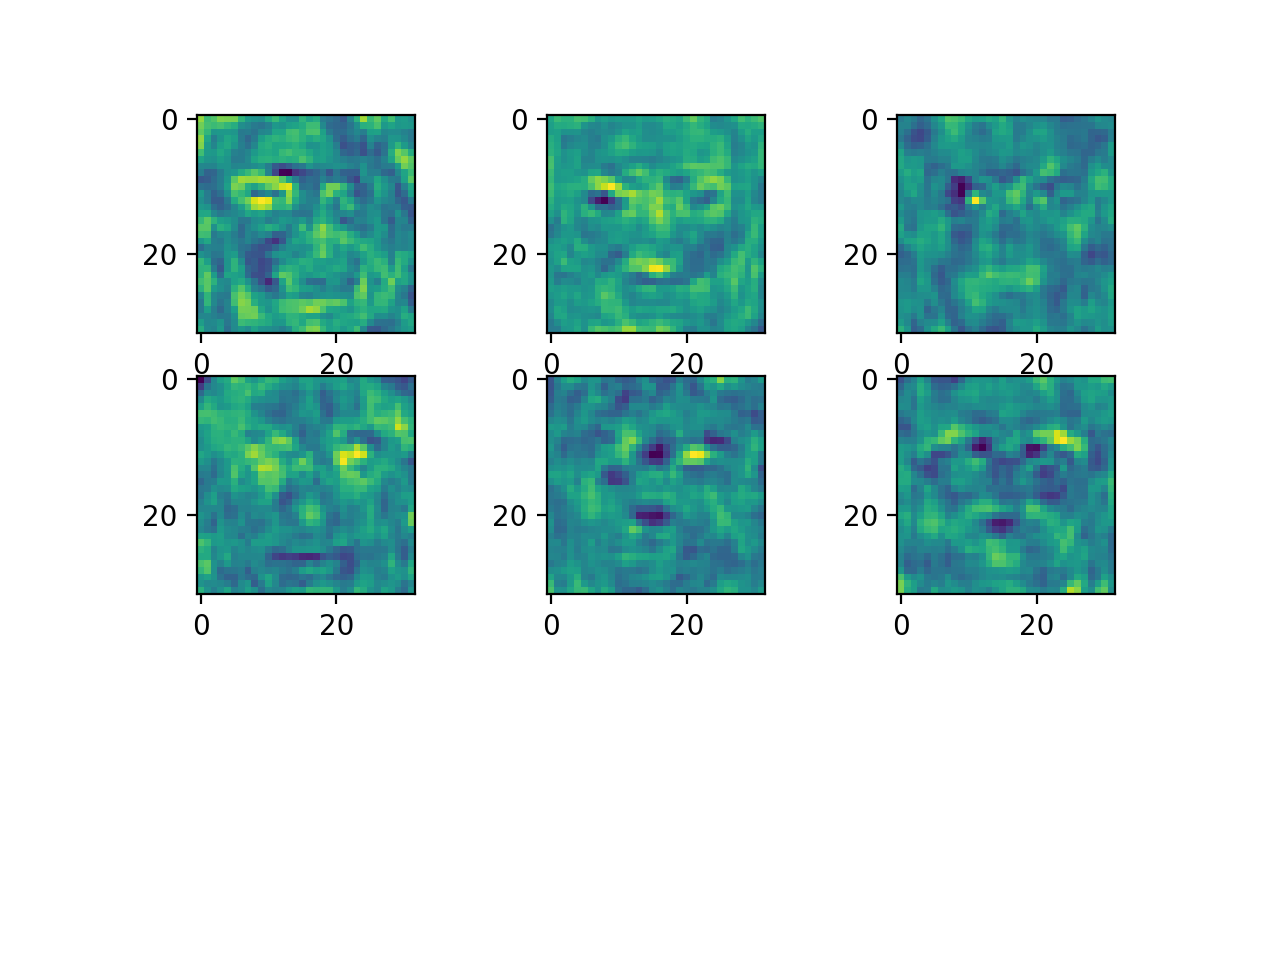
\includegraphics[scale = 0.6]{part8.png}\\

Want to compute $I(Y, x_i)$ for the first split of the decision tree. Therefore, $x_i$ is the keyword "the". Y is either real or fake.\\

First compute the entropy:\\
\(H(Y) = \sum_v - P(Y=v)log_2 P(Y=v)\)\\
\hspace*{27pt}\(= - P(Y = fake)log_2 P(Y=fake) - P(Y = real)log_2 P(Y=real)\)\\
\hspace*{27pt}\(= - \frac{908}{2285}log_2 \frac{908}{2285} - \frac{1377}{2285}log_2 P(\frac{1377}{2285})\)\\
\hspace*{27pt}\(\approx 0.529 + 0.4403\)\\
\hspace*{27pt}\(= 0.9693\)\\

\(H(Y|x_i = \neg the) = - \frac{661}{1931}log_2 \frac{661}{1931} - \frac{1270}{1931}log_2 P(\frac{1270}{1931})\)\\
\hspace*{75pt}\(\approx 0.9270\)\\

\(H(Y|x_i = the) = - \frac{247}{354}log_2 \frac{247}{354} - \frac{107}{354}log_2 P(\frac{107}{354})\)\\
\hspace*{67pt}\(\approx 0.8840\)\\

Also,\\
\(P(x_i = \neg the) = 1931/2285 \approx 0.8451\)\\
\(P(x_i = the) = 354/2285 \approx 0.1549\)\\

Then, the mutual information is:\\
\(I(Y, x_i) = H(Y) - \sum_x P(x_i = x)H(Y|x_i = x)\)\\
\hspace*{35pt}\(= H(Y) - [P(x_i = the)H(Y|x_i = the) + P(x_i = \neg the)H(Y|x_i = \neg the)]\)\\
\hspace*{35pt}\(= 0.9693 - (0.1549 \times 0.8840 + 0.8451 \times 0.9270)\)\\
\hspace*{35pt}\(= 0.0489607\)

\clearpage
\subsection{Part B}
Below is the code we used to obtain the information required to compute \(I(Y, x_j)\), where the keyword is 'trumps':\\
\begin{lstlisting}
def part8b():
    real_with_word = []
    for headline in train_real:
        if "trumps" in list(headline):
            real_with_word.append(headline)
            
    with_word_real_split = len(real_with_word)
    without_word_real_split = len(train_real) - with_word_real_split
    
    fake_with_word = []
    for headline in train_fake:
        if "trumps" in list(headline):
            fake_with_word.append(headline)
    
    with_word_fake_split = len(fake_with_word)
    without_word_fake_split = len(train_fake) - with_word_fake_split
    
    print("Number of total headlines: " + str(len(train_real) + len(train_fake)))
    print("Number of initial fake headlines: " + str(len(train_fake)))
    print("Number of initial real headlines: " + str(len(train_real)))
    print("\n")
    print("Number of headlines without word 'trumps': " +
    str(without_word_fake_split + without_word_real_split))
    print("Number of fake headlines in the dataset without word 'trumps': " +
    str(without_word_fake_split))
    print("Number of real headlines in the dataset without word 'trumps': " +
    str(without_word_real_split))
    print("\n")
    print("Number of headlines with word 'trumps': " + str(with_word_fake_split +
    with_word_real_split))
    print("Number of fake headlines in the dataset with word 'trumps': " +
    str(with_word_fake_split))
    print("Number of real headlines in the dataset with word 'trumps': " +
    str(with_word_real_split))
\end{lstlisting}

The output is:\\
Number of total headlines: 2285\\
Number of initial fake headlines: 908\\
Number of initial real headlines: 1377\\

Number of headlines without word 'trumps': 2132\\
Number of fake headlines in the dataset without word 'trumps': 905\\
Number of real headlines in the dataset without word 'trumps': 1227\\

Number of headlines with word 'trumps': 153\\
Number of fake headlines in the dataset with word 'trumps': 3\\
Number of real headlines in the dataset with word 'trumps': 150\\

Use the same method to compute \(I(Y, x_j)\) as how we computed \(I(Y, x_i)\) in part A:\\

First compute the entropy:\\
\(H(Y) = \sum_v - P(Y=v)log_2 P(Y=v)\)\\
\hspace*{27pt}\(= - P(Y = fake)log_2 P(Y=fake) - P(Y = real)log_2 P(Y=real)\)\\
\hspace*{27pt}\(= - \frac{908}{2285}log_2 \frac{908}{2285} - \frac{1377}{2285}log_2 P(\frac{1377}{2285})\)\\
\hspace*{27pt}\(\approx 0.529 + 0.4403\)\\
\hspace*{27pt}\(= 0.9693\)\\

\(H(Y|x_j = \neg trumps) = - \frac{905}{2132}log_2 \frac{905}{2132} - \frac{1227}{2132}log_2 P(\frac{1227}{2132})\)\\
\hspace*{93pt}\(\approx 0.9835\)\\

\(H(Y|x_j = trumps) = - \frac{3}{153}log_2 \frac{3}{153} - \frac{150}{153}log_2 P(\frac{150}{153})\)\\
\hspace*{87pt}\(\approx 0.1392\)\\

Also,\\
\(P(x_j = \neg trumps) = 2132/2285 \approx 0.9331\)\\
\(P(x_j = trumps) = 153/2285 \approx 0.0669\)\\

Then, the mutual information is:\\
\(I(Y, x_j) = H(Y) - \sum_x P(x_j = x)H(Y|x_j = x)\)\\
\hspace*{35pt}\(= H(Y) - [P(x_j = trumps)H(Y|x_j = trumps) + P(x_j = \neg trumps)H(Y|x_j = \neg trumps)]\)\\
\hspace*{35pt}\(= 0.9693 - (0.0669 \times 0.1392 + 0.9331 \times 0.9835)\)\\
\hspace*{35pt}\(= 0.04228367\)\\

The mutual information obtained in part B is slightly smaller than part A. This might be because 'trumps' is one of the words in the first layer of the original decision tree. However, it's better for the mutual information to be bigger. Therefore, it's better to keep word 'the' as the first split rather than using word 'trumps'.\\

\end{homeworkProblem}
\clearpage

%----------------------------------------------------------------------------------------


\end{document}